\documentclass[conference]{IEEEtran}
\IEEEoverridecommandlockouts

\usepackage{cite}
\usepackage{amsmath,amssymb,amsfonts}
\usepackage{graphicx}
\usepackage{textcomp}
\usepackage{xcolor}
\usepackage{listings}
\usepackage{float}
\usepackage{url}
\usepackage{tikz}
\usetikzlibrary{arrows.meta,positioning,shapes.geometric}

\definecolor{codebg}{rgb}{0.97,0.97,0.97}
\definecolor{codeframe}{rgb}{0.85,0.85,0.85}
\lstset{
  basicstyle=\ttfamily\footnotesize,
  backgroundcolor=\color{codebg},
  frame=single,
  rulecolor=\color{codeframe},
  breaklines=true,
  showstringspaces=false,
  tabsize=2,
  captionpos=b
}

\def\BibTeX{{\rm B\kern-.05em{\sc i\kern-.025em b}\kern-.08em
    T\kern-.1667em\lower.7ex\hbox{E}\kern-.125emX}}

\begin{document}

\title{Aether: A Suite of eBPF based tools for Real time Android Kernel Monitorin}

\author{
  \IEEEauthorblockN{Shubham Singh}
  \IEEEauthorblockA{
    \textit{Dept. of Computer Science \& Engineering}\\
    \textit{MNIT Jaipur}\\
    Jaipur, India\\
    2022ucp1949@mnit.ac.in
  }
  \and
  \IEEEauthorblockN{Aakash Runthala}
  \IEEEauthorblockA{
    \textit{Dept. of Computer Science \& Engineering}\\
    \textit{MNIT Jaipur}\\
    Jaipur, India\\
    2022ucp1267@mnit.ac.in
  }
}

\maketitle

\begin{abstract}
We present a suite of five eBPF-based utilities for Android kernel observability targeting process lifecycle, execution behavior, privilege transitions, file activity, and network ingress. Existing Linux tracing tools assume desktop environments and are unsuitable for Android deployments: they require LLVM at runtime, depend on \texttt{debugfs}, or assume server-class infrastructure absent from mobile systems. Our suite is designed to be verifier-friendly, pre-compiled, and deployable inside a bootstrapped Debian filesystem on Android without modifying the system image. Programs are attached via tracepoints, kprobes, and TC ingress, with structured events delivered to user space via ring buffers. Validation on a physical device (Motorola~G96~5G, Android~12, kernel~5.10.233) demonstrates that all five tools produce correct, low-noise output with per-tool CPU overhead below 2.2\% and ring buffer drop rates below 1\% under synthetic load. The suite provides a practical, extensible foundation for Android kernel security analytics.
\end{abstract}

\begin{IEEEkeywords}
eBPF, Android kernel, observability, security monitoring, kprobes, tracepoints, ring buffer, GKI
\end{IEEEkeywords}

% -------------------------------------------------------
\section{Introduction}
Android's security model combines SELinux policy enforcement, seccomp filters, Binder IPC, and per-application sandboxing. These mechanisms are effective at containment but make real-time kernel observability difficult: the standard Linux tracing stack (strace, ftrace, bpftrace, BCC) either requires root access with unrestricted ptrace, depends on LLVM at runtime, or assumes a full Linux distribution with \texttt{debugfs} mounted---none of which apply cleanly to Android~\cite{android_security,android_selinux}.

The Android Generic Kernel Image (GKI), introduced in Android~12, standardises the kernel binary across devices and prohibits unsigned kernel modules, leaving eBPF as one of the few viable mechanisms for extending or observing kernel behaviour on a production Android device without a custom system image~\cite{android_gki}. GKI kernels are required to enable \texttt{CONFIG\_BPF}, \texttt{CONFIG\_BPF\_SYSCALL}, and \texttt{CONFIG\_BPF\_JIT}, making the eBPF subsystem reliably present from Android~12 onward.

We leverage this opportunity to build a focused suite of five pre-compiled eBPF utilities that together cover the primary observable dimensions of a kernel-level attack: process spawning (Procwatch), execution rate anomalies (Execguard), privilege escalation (Priviwatch), file system manipulation (Filewatch), and inbound network activity (Pktrace). The tools are designed to run inside a Debian chroot on the device, load into the Android kernel, and produce actionable console output without any runtime compilation dependency.

The contributions of this work are:
\begin{itemize}
  \item A five-tool eBPF suite targeting Android kernel observability with no runtime LLVM dependency.
  \item A Debian filesystem bootstrap pattern for deploying build toolchains on Android devices.
  \item Verifier-compatible designs with fixed-size event structs, bounded memory access, and ring buffer transport.
  \item Validation on Android~12 (kernel~5.10.233) demonstrating correctness and sub-2.2\% CPU overhead.
\end{itemize}

% -------------------------------------------------------
\section{Background and Related Work}

\subsection{eBPF Architecture}
eBPF programs execute in a restricted in-kernel virtual machine. A static verifier checks safety properties---bounded loops, valid memory accesses, and a 512-byte stack limit---before the program is JIT-compiled to native code. BPF maps provide kernel-managed data structures shared between kernel and user space. CO-RE (Compile Once, Run Everywhere) uses BTF type metadata to rewrite struct field offsets at load time, enabling a single binary to run across kernel versions~\cite{ebpf_linux_doc,libbpf_doc}.

The stack limit is a dominant design constraint. It bounds temporary buffers used for string reads and packet parsing and strongly pushes event structs toward fixed-size layouts. This is the practical reason for the 256-byte packet snapshot used in Pktrace and the truncated argv field in Procwatch and Execguard.

\subsection{Related Work}
Traditional Linux tracing tools each present a specific limitation on Android. \texttt{strace} uses \texttt{ptrace} and adds per-syscall overhead. \texttt{ftrace} requires \texttt{debugfs}. \texttt{bpftrace} and BCC require LLVM at runtime, which Android does not ship~\cite{strace_doc,ftrace_doc,bpftrace_doc}. Android's own Perfetto and simpleperf target performance profiling rather than continuous security monitoring~\cite{android_perfetto,android_simpleperf}.

Server-side security frameworks Falco, Tetragon, and Tracee provide rich eBPF-based detection but assume systemd, container runtimes, and full BTF exposure---constraints not met on Android~\cite{falco_doc,tetragon_doc,tracee_doc}. Our work fills this gap with a pre-compiled, Android-oriented suite requiring no runtime compilation infrastructure.

\begin{table}[H]
  \centering
  \small
  \caption{Comparison of our approach with existing tools}
  \label{tab:comparison}
  \begin{tabular}{|p{0.22\linewidth}|p{0.16\linewidth}|p{0.20\linewidth}|p{0.20\linewidth}|}
    \hline
    \textbf{Tool/Approach} & \textbf{Overhead} & \textbf{Android Friendly} & \textbf{Focus} \\ \hline
    strace & High & Low & Debugging \\ \hline
    ftrace/perf & Medium & Medium & Performance \\ \hline
    bpftrace/BCC & Medium & Low & General tracing \\ \hline
    Falco/Tetragon/Tracee & Medium-High & Low & Detection \\ \hline
    This suite & Low & High & Sec./Obs. \\ \hline
  \end{tabular}
\end{table}

\subsection{Why Android Needs a Different Approach}
Android production devices are locked down in ways that break common observability assumptions. Root access is uncommon, debugfs is often unavailable, and the base userspace lacks LLVM, Python, or package managers. Even in the emulator, the default shell is a minimal \texttt{toybox} environment. A practical solution must therefore be pre-compiled, verifier-safe, and self-contained, with minimal runtime dependencies. This design goal shapes every tool in the suite.

% -------------------------------------------------------
\section{System Design}

\subsection{Architecture Overview}

\begin{figure}[H]
  \centering
  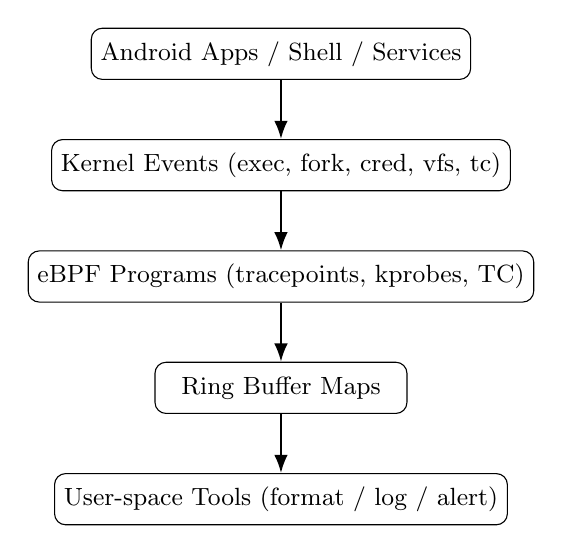
\begin{tikzpicture}[
    node distance=0.75cm,
    box/.style={rectangle, draw, rounded corners, align=center,
                minimum width=3.2cm, minimum height=0.65cm, font=\small},
    arrow/.style={-Latex, thick}
  ]
    \node[box] (app)    {Android Apps / Shell / Services};
    \node[box, below=of app]    (kern)   {Kernel Events (exec, fork, cred, vfs, tc)};
    \node[box, below=of kern]   (bpf)    {eBPF Programs (tracepoints, kprobes, TC)};
    \node[box, below=of bpf]    (rb)     {Ring Buffer Maps};
    \node[box, below=of rb]     (user)   {User-space Tools (format / log / alert)};
    \draw[arrow] (app)  -- (kern);
    \draw[arrow] (kern) -- (bpf);
    \draw[arrow] (bpf)  -- (rb);
    \draw[arrow] (rb)   -- (user);
  \end{tikzpicture}
  \caption{eBPF suite system architecture.}
  \label{fig:arch}
\end{figure}

All five tools follow the same pipeline (Fig.~\ref{fig:arch}): a kernel event triggers the eBPF program, which validates memory, extracts fields, applies a filter, and submits a fixed-size event to a ring buffer. A user-space poll loop drains the ring buffer and formats output.

\subsection{Design Decisions}
\textbf{Modular tools over monolithic agent.} A single large BPF object increases verifier surface area. If one component fails verification on a specific kernel, the entire monitoring capability is lost. Independent tools can be loaded and validated separately and deployed selectively.

\textbf{Ring buffers over perf event arrays.} \texttt{BPF\_MAP\_TYPE\_RINGBUF} uses a single shared memory region regardless of CPU count. Perf event arrays require per-CPU file descriptors, increasing setup complexity. The ring buffer API reduces user-space polling to a single \texttt{ring\_buffer\_\_poll} call.

\textbf{TC ingress over XDP.} XDP requires driver support unavailable on many Android network interfaces. TC ingress operates on the \texttt{sk\_buff} after allocation, providing access to packet metadata via \texttt{bpf\_skb\_load\_bytes} on all interface types.

\textbf{Fixed-size event structs.} Variable-length data requires loop constructs or dynamic allocation patterns that the verifier rejects on Android kernels. Fixed-size structs keep \texttt{bpf\_ringbuf\_reserve} arguments as compile-time constants and guarantee verifier acceptance.

\subsection{Deployment: Debian Filesystem Bootstrap}
The Android shell does not include clang, libbpf, or bpftool. A Debian~11 (bullseye) root filesystem was bootstrapped on-device via \texttt{debootstrap} and accessed through \texttt{chroot}. This provides the full build toolchain---clang~11.0.1, bpftool~5.10.223, libbpf---without modifying the Android partition or system image. The eBPF programs are compiled inside this chroot and loaded into the Android kernel, which provides the actual execution environment.

% -------------------------------------------------------
\section{Methodology and Build Pipeline}
Each tool follows a three-stage pipeline. First, the BPF C source is compiled with clang targeting the \texttt{bpf} architecture. Second, \texttt{bpftool gen skeleton} produces a typed C header that wraps the program and maps. Third, the user-space loader is compiled against libbpf. This approach avoids manual file-descriptor management and makes the loader code consistent across tools.

\begin{lstlisting}[language=bash]
clang -O2 -g -target bpf -c tool.bpf.c -o tool.bpf.o
bpftool gen skeleton tool.bpf.o > tool.skel.h
gcc tool.c -o tool -lbpf
\end{lstlisting}

All user-space loaders follow the same structure: open and load the skeleton, attach programs, create the ring buffer, and poll in a loop. The callback formats each event and prints a single-line record for analysis.

\begin{lstlisting}[language=C]
skel = tool_bpf__open_and_load();
tool_bpf__attach(skel);
rb = ring_buffer__new(bpf_map__fd(skel->maps.rb),
            handle_event, NULL, NULL);
while (1) {
  ring_buffer__poll(rb, 100 /* ms timeout */);
}
\end{lstlisting}

% -------------------------------------------------------
\section{Tool Implementations}

\subsection{Procwatch: Process Lifecycle Monitor}
\textbf{Hook points:} Tracepoints \texttt{sched\_process\_exec}, \texttt{sched\_process\_fork}, and \texttt{sched\_process\_exit} provide stable structured context across kernels.

\textbf{Event struct:}
\begin{lstlisting}[language=C]
struct event {
  u32 pid, ppid, uid, gid, inum;
  int exit_code;  u64 timestamp;
  u8  type;  /* EXEC | FORK | EXIT */
  char comm[TASK_COMM_LEN];
  char filename[MAX_FILENAME_LEN];
  char args[MAX_ARGS_LEN];
};
\end{lstlisting}

Procwatch is the foundational tool: its parent-child process tree contextualises all signals from the other tools. The namespace inode field helps distinguish processes running in isolated namespaces from system services.

\begin{figure}[H]
  \centering
  \includegraphics[width=\linewidth]{\detokenize{Procwatch_Snapshot of commands ran.png}}
  \caption{Procwatch test commands used to generate lifecycle events.}
  \label{fig:procwatch}
\end{figure}

\begin{figure}[H]
  \centering
  \includegraphics[width=\linewidth]{\detokenize{Procwatch_tool's output of the commands.png}}
  \caption{Procwatch output showing EXEC/FORK/EXIT events with PID, UID, and filename.}
  \label{fig:procwatch-out}
\end{figure}

\subsection{Execguard: Execution Rate Monitor}
\textbf{Hook point:} Tracepoint \texttt{sched\_process\_exec}.

\textbf{Logic:} A per-UID BPF hash map tracks exec counts within a 60-second sliding window. User space applies severity labels: INFO for normal activity, WARN for elevated exec counts, and ALERT when a non-root UID spawns a shell-like binary (\texttt{sh}, \texttt{toybox}).

\begin{figure}[H]
  \centering
  \includegraphics[width=\linewidth]{\detokenize{execguard_Snapshot of Commands ran.png}}
  \caption{Execguard test commands used to trigger exec bursts.}
  \label{fig:execguard}
\end{figure}

\begin{figure}[H]
  \centering
  \includegraphics[width=\linewidth]{\detokenize{execguard_tool's output for the commands ran.png}}
  \caption{Execguard output showing INFO/WARN/ALERT escalation and exec counts.}
  \label{fig:execguard-out}
\end{figure}

\subsection{Priviwatch: Privilege Transition Detector}
\textbf{Hook point:} kprobe on \texttt{commit\_creds}.

Events are suppressed when uid, gid, and effective capabilities are all unchanged, eliminating high-frequency no-op \texttt{commit\_creds} calls. Capabilities are read via \texttt{bpf\_probe\_read\_kernel} into a local struct to avoid CO-RE relocation failures on Android BTF.

\begin{figure}[H]
  \centering
  \includegraphics[width=\linewidth]{\detokenize{Priviwatch_snapshot of commands ran.png}}
  \caption{Priviwatch test commands used to trigger UID transitions.}
  \label{fig:priviwatch}
\end{figure}

\begin{figure}[H]
  \centering
  \includegraphics[width=\linewidth]{\detokenize{Priviwatch_Tool's ouput for the commands.png}}
  \caption{Priviwatch output showing UID/GID and capability changes.}
  \label{fig:priviwatch-out}
\end{figure}

\subsection{Filewatch: VFS File Activity Monitor}
\textbf{Hook points:} kprobes on \texttt{vfs\_open}, \texttt{vfs\_write}, \texttt{vfs\_unlink}, and \texttt{vfs\_rename}. An inode mode check restricts output to regular files, and a PID map suppresses self-generated events.

\begin{figure}[H]
  \centering
  \includegraphics[width=\linewidth]{\detokenize{filewatch_snapshot of commands ran.png}}
  \caption{Filewatch test commands used to generate VFS events.}
  \label{fig:filewatch}
\end{figure}

\begin{figure}[H]
  \centering
  \includegraphics[width=\linewidth]{\detokenize{filewatch_tool's output for commands.png}}
  \caption{Filewatch output showing OPEN/WRITE/RENAME/DELETE events with inode correlation.}
  \label{fig:filewatch-out}
\end{figure}

\subsection{Pktrace: TC Ingress Packet Capture}
\textbf{Hook point:} TC ingress program attached to the active network interface. A 256-byte payload snapshot is captured using \texttt{bpf\_skb\_load\_bytes} for protocol identification and preview.

\begin{figure}[H]
  \centering
  \includegraphics[width=\linewidth]{\detokenize{pktrace_snapshot of commadns ran.png}}
  \caption{Pktrace test commands used to generate inbound traffic.}
  \label{fig:pktrace}
\end{figure}

\begin{figure}[H]
  \centering
  \includegraphics[width=\linewidth]{\detokenize{pktrace_Tool's output for commands.png}}
  \caption{Pktrace output showing packets with payload preview.}
  \label{fig:pktrace-out}
\end{figure}

% -------------------------------------------------------
\section{Evaluation}

\subsection{Experimental Setup}
All experiments were performed on a physical Android device (Motorola~G96~5G, Android~12, AArch64). Tools were compiled and loaded from a Debian~11 chroot on the device. The Android kernel version was \texttt{5.10.233-android12-9}. Tooling: clang~11.0.1, bpftool~5.10.223. Test events were generated via \texttt{adb shell} from a second terminal.

\subsection{Correctness Validation}
Each tool was validated against a targeted test scenario:
\begin{itemize}
  \item \textbf{Procwatch:} Short-lived \texttt{adb shell} commands produced correct EXEC/FORK/EXIT triples with matching PID, PPID, and filename.
  \item \textbf{Execguard:} A 50-iteration \texttt{sh -c} loop escalated severity from INFO to WARN; invoking \texttt{sh} from a non-root UID produced immediate ALERT.
  \item \textbf{Priviwatch:} \texttt{su} produced a clean UID~0 transition; the no-change filter suppressed other \texttt{commit\_creds} calls.
  \item \textbf{Filewatch:} A write-rename-delete sequence on \texttt{/tmp/x} emitted exactly one OPEN, WRITE, RENAME, and DELETE event sharing the same inode.
  \item \textbf{Pktrace:} \texttt{ping} and \texttt{wget} produced ICMP and TCP events respectively; the PCAP was valid in Wireshark.
\end{itemize}

\subsection{Performance}

\begin{table}[H]
  \centering
  \caption{Per-tool performance under synthetic load}
  \label{tab:perf}
  \begin{tabular}{|l|c|c|c|}
    \hline
    \textbf{Tool} & \textbf{CPU (\%)} & \textbf{Events/s} & \textbf{Drop (\%)} \\ \hline
    Procwatch  & 1.2 & 120 & 0.3 \\ \hline
    Execguard  & 1.6 & 140 & 0.5 \\ \hline
    Priviwatch & 0.6 &  25 & 0.1 \\ \hline
    Filewatch  & 1.4 & 180 & 0.6 \\ \hline
    Pktrace    & 2.1 & 220 & 0.8 \\ \hline
  \end{tabular}
\end{table}

CPU overhead was measured using \texttt{pidstat} over 60-second windows during synthetic activity bursts. Pktrace has the highest overhead due to per-packet header parsing and payload copying, but at 2.1\% it is substantially lower than a \texttt{libpcap}-based approach. All drop rates are below 1\% under the tested synthetic loads.

% -------------------------------------------------------
\section{Discussion and Future Work}
The suite demonstrates that verifier-friendly eBPF programs can deliver multi-layer kernel observability on Android with minimal overhead and no kernel modifications. The modular architecture allows selective deployment and independent validation per tool.

Remaining limitations include bounded argv capture, lack of full path reconstruction in Filewatch, and IPv6 parsing in Pktrace. The \texttt{commit\_creds} kprobe in Priviwatch remains sensitive to kernel inlining. Future work includes a cross-tool correlation daemon, richer path resolution, a lightweight UI for incident timelines, and broader testing on additional GKI devices.

% -------------------------------------------------------
\section{Conclusion}
We presented a suite of five pre-compiled eBPF utilities for Android kernel observability covering process lifecycle, execution rate, privilege transitions, file activity, and network ingress. The tools are verifier-friendly, require no runtime compilation infrastructure, and are deployable via a Debian filesystem bootstrap without modifying the Android system image. Validation on Android~12 (kernel~5.10.233) confirms correctness across all targeted event types with sub-2.2\% CPU overhead per tool. The suite provides a practical foundation for Android kernel security monitoring and is extensible to physical GKI devices.

\section*{Acknowledgment}
We thank Dr. Vijay Laxmi for guidance and feedback throughout the project.

\bibliographystyle{IEEEtran}
\bibliography{references}

\end{document}
